\documentclass[a4paper,12pt]{extarticle}
\usepackage{geometry,microtype,mathtools,amsthm,amssymb,enumitem}
\usepackage[utf8]{inputenc}
\usepackage[font=small,labelfont=bf]{caption}
\theoremstyle{definition}
\newcommand{\R}{\mathbb{R}} \newcommand{\Q}{\mathbb{Q}} \newcommand{\Z}{\mathbb{Z}} \newcommand{\N}{\mathbb{N}} \newcommand{\myskip}{\par\null\par} \renewcommand\qedsymbol{QED} \renewcommand{\leq}{\leqslant}\renewcommand{\geq}{\geqslant}
\newtheorem*{theorem}{Theorem}
\title{Math 431 Final} 
\author{Theo Koss}
\date{December 2022} 
\begin{document}
    \maketitle
    \section*{Problem 1}
    Let $G$ be a group, and suppose that $|g|\leq2$ for all $g\in G$. Show that $G$ is abelian, and if $G$ is finite, that $G$ is a direct sum of copies of $\Z_2$, so that $|G|=2^n$ for some $n\in\N\cup\{0\}$.
    \begin{proof}
    Consider $g,h\in G$ both with order 2. That is, $g^2=e$ and $h^2=e$. We must show that $gh=hg$. \begin{align*}
       e&=(gh)^2\\
       &=ghgh
    \end{align*}Multiply by g on the left, and h on the right.\begin{align*}
        g\cdot e\cdot h&= g\cdot ghgh\cdot h\\
        gh &= e\cdot h\cdot g\cdot e\\
        gh &=hg \\
    \end{align*} Therefore $G$ is abelian.
    \myskip Now assume $G$ is finite, so we can enumerate all of the elements, label the identity elements $e_i$ and every other element $g_i$. Where $I$ is the indexing set. Then for each pair of $e_i,g_i$, define a subgroup of $G$ called $H_i$. $H_i=\{e_i,g_i\}$, it remains to show that $H_i\cong\Z_2$. Define an isomorphism $\phi:\Z_2\to H_i$, which maps $0\mapsto e_i$ and $1\mapsto g_i$.\myskip Then $$G\cong\bigoplus_{i\in I}H_i\cong\bigoplus_{i\in I}\Z_2$$ and $|G|=2^{|I|}$. So $G$ is isomorphic to a direct sum of copies of $\Z_2$ and $|G|=2^n$ for some natural number $n$.
    \end{proof}
    \section*{Problem 2}
    Let $G$ be a group of order 6.
    \begin{enumerate}[label=(\alph*)]
        \item Show that $G$ must contain an element $a$ with $|a|=3$.\myskip Recall that for any group of even order, there can exist only an odd number of elements of order 2. Thus $G$ must have some element with order 3.
        \item Show that $G$ must contain an element $b\in G\backslash\langle a\rangle$ such that $b^2\in\langle a\rangle$. Show that we can assume that $|b|=2$, and that $G=\langle a\rangle\cup b\langle a\rangle=\{e,a,a^2,b,ba,ba^2\}$.\myskip We know $|a|=3$, so by Lagrange's theorem, the number of left cosets of $\langle a\rangle$ is 2, and they must be $e\langle a\rangle$ and $b\langle a\rangle$. Furthermore, these coefficients must also determine a group, that is, $\{e,b\}$ must be a group, this means that $|b|=2$, and $G$ is partitioned into cosets by $\langle a\rangle$.
        \item Show that either $ab=ba$ or $ab=ba^2$, and that in the first of these cases, $G\cong\Z_6$ while in the second, $G\cong S_3$. \myskip Since $G=\{e,a,a^2,b,ba,ba^2\}$, $ab$ must be equal to one of the elements of the group, as there are already 6 unique elements. If $ab=e$, then $a=b^{-1}$, but since $|b|=2$, this implies that $a=b$, which is impossible. $ab=a$ implies that $b$ is the identity, which is also not true. Similarly, $ab=b$ and $ab=b^2$ can not be true. That leaves us with 2 cases, either $ab=ba$ or $ab=ba^2$.\begin{enumerate}[label=\roman*.]
            \item In the first case, where $ab=ba$, any product of $a$'s and $b$'s can be rewritten as $a^ib^j$, where $i\in\Z_2$ and $j\in\Z_3$. This implies that $G\cong\Z_6$.
            \item In the second, we will see that there exists an isomorphism $\phi:G\to S_3$, the group of symmetries of a regular $n$-gon. This isomorphism sends $a$ to the ``$60^{\circ}$ rotation'' operation, and $b$ to the ``reflection through a vertex'' operation. To see that this is indeed an isomorphism, notice $|a|=3$, and 3 $60^{\circ}$ rotations gives $e$, so $|\phi(a)|=3$. Also $|b|=2$, and 2 reflections through a vertex gives $e$, so $|b|=|\phi(b)|$. So, $|x|=|\phi(x)|,\ \forall x\in G$, so $\phi$ is an isomorphism.
            \end{enumerate}
        \end{enumerate}
        \section*{Problem 3}
        Consider the matrices $$A=\begin{pmatrix}
        0 & 1\\
        -1 & 0\\
        \end{pmatrix}\text{and }B=\begin{pmatrix}
        0 & i\\
        i & 0\\
        \end{pmatrix}$$ Where $i^2=-1$. Show that $A^2=B^2=-I_{2\times2}$, that $A^4=B^4=I_{2\times2}$, and that $BA=A^3B$. Conclude that every element of the matrix group $Q_8=\langle A,B\rangle$ generated by $A$ and $B$ can be written in the form $A^iB^j$, and that $Q_8$ is in fact a non-abelian group of order 8.\myskip\begin{align*}
            A^2&=\begin{pmatrix}
        0 & 1\\
        -1 & 0\\
        \end{pmatrix}\cdot\begin{pmatrix}
        0 & 1\\
        -1 & 0\\
        \end{pmatrix}=\begin{pmatrix}
        0 & -1\\
        -1 & 0\\
        \end{pmatrix}=-I_{2\times2}\\
        B^2&=\begin{pmatrix}
        0 & i\\
        i & 0\\
        \end{pmatrix}\cdot\begin{pmatrix}
        0 & i\\
        i & 0\\
        \end{pmatrix}=\begin{pmatrix}
        0 & -1\\
        -1 & 0\\
        \end{pmatrix}=-I_{2\times2}
        \end{align*}
        \begin{align*}
            A^4&=\begin{pmatrix}
        0 & 1\\
        -1 & 0\\
        \end{pmatrix}\cdot\begin{pmatrix}
        0 & 1\\
        -1 & 0\\
        \end{pmatrix}\cdot\begin{pmatrix}
        0 & 1\\
        -1 & 0\\
        \end{pmatrix}\cdot\begin{pmatrix}
        0 & 1\\
        -1 & 0\\
        \end{pmatrix}=\begin{pmatrix}
        0 & 1\\
        1 & 0\\
        \end{pmatrix}=I_{2\times2}\\
        B^4&=\begin{pmatrix}
        0 & i\\
        i & 0\\
        \end{pmatrix}\cdot\begin{pmatrix}
        0 & i\\
        i & 0\\
        \end{pmatrix}\cdot\begin{pmatrix}
        0 & i\\
        i & 0\\
        \end{pmatrix}\cdot\begin{pmatrix}
        0 & i\\
        i & 0\\
        \end{pmatrix}=\begin{pmatrix}
        0 & 1\\
        1 & 0\\
        \end{pmatrix}=I_{2\times2}
        \end{align*}
        \begin{align*}
            BA&=\begin{pmatrix}
        0 & i\\
        i & 0\\
        \end{pmatrix}\cdot\begin{pmatrix}
        0 & 1\\
        -1 & 0\\
        \end{pmatrix}=\begin{pmatrix}
        -i & 0\\
        0 & i\\
        \end{pmatrix}=A^3B\\
        &\neq AB
        \end{align*}
        $Q_8=\langle A,B\rangle$ can be written as $A^iB^j$ where $i\in\Z_4$ and $j\in\Z_4$, since $A$ and $B$ both have order 4.
        \section*{Problem 4}
        Let $G$ be a group of order 8. Note that if $G$ contains an element of order 8, then $G\cong\Z_8$, while if every non-identity element of $G$ has order 2, then $G\cong\Z_2\times\Z_2\times\Z_2$. Suppose for now that neither of those cases occurs.
        \begin{enumerate}
            \item Show that $G$ must contain an element $a$ with $|a|=4$, and an element $b\in G\backslash\langle a\rangle$ such that $b^2=\langle a\rangle$. Show, in addition, that either $b^2=e$ or $b^2=a^2$.\begin{proof}
            Let $G=\{e,a,a^2,a^3,b,ba,ba^2,ba^3\}$, then, we can partition $G$ into cosets of order 4, that is, $G=e\langle a\rangle\cup b\langle a\rangle$, and thus, $\{e,b\}$ defines a group, so $|b|=2$ and $b^2=e$.
            \end{proof}
            \item Explain why $bab^{-1}\in\langle a\rangle$, and show that either $bab^{-1}=a$ or $bab^{-1}=a^3$. In the first case, show that $G\cong\Z_4\times\Z_2$; in the second case, show that $G\cong D_4$ if $|b|=2$, and $D\cong Q_8$ if $|b|=4$. NOT SURE
            \item Conclude that there are exactly 5 non-isomorphic groups of order 8.\myskip There is $\Z_8$, $\Z_2\times\Z_2\times\Z_2$, $\Z_4\times\Z_2$, $D_4$ and $Q_8$. They are all non-isomorphic to one another.
        \end{enumerate}
        \section*{Problem 5}
        Classify the groups with $1\leq|G|\leq8$.
        \begin{itemize}
            \item $|G|=1$\begin{itemize}
                \item $\{e\}$
            \end{itemize}
            \item $|G|=2$\begin{itemize}
                \item $\Z_2$
            \end{itemize}
            \item $|G|=3$\begin{itemize}
                \item $\Z_3$
            \end{itemize}
            \item $|G|=4$\begin{itemize}
                \item $\Z_4$
                \item $\Z_2\times\Z_2$
            \end{itemize}
            \item $|G|=5$\begin{itemize}
                \item $\Z_5$
            \end{itemize}
            \item $|G|=6$\begin{itemize}
                \item $\Z_6$
                \item $S_3$
            \end{itemize}
            \item $|G|=7$\begin{itemize}
                \item $\Z_7$
            \end{itemize}
            \item $|G|=8$\begin{itemize}
                \item $\Z_8$
                \item $\Z_2\times\Z_2\times\Z_2$
                \item $\Z_4\times\Z_2$
                \item $D_4$
                \item $Q_8$
            \end{itemize}
        \end{itemize}
        \section*{Problem 6}
        Verify that $E(n)$ is indeed a group under the stated operation, and that every element of $E(n)$ is both an isometry of $R^n$ and a bijection.\begin{proof}
        We must show: \begin{itemize}
            \item Associativity: The group operation $$(A,\textbf{v})(B,\textbf{w})=(AB,A\textbf{w}+\textbf{v})$$ Is just a combination of matrix multiplication and vector addition, both of which are associative.
            \item Identity: The identity is the function $(I,\textbf{0})$, because $(I,0)(A,v)=(IA,Iv)=(A,v)$.
            \item Inverses: For $(A,v)$, the inverse is $(A^{-1},-v)$, since $(A,v)(A^{-1},-v)=(I,0)$.
        \end{itemize} Therefore $E(n)$ is a group.\myskip Consider some $x,y$. $f(x)=A\textbf{x}+\textbf{v}$, and $f(y)=A\textbf{y}+\textbf{v}$, for some orthogonal matrix $A$ and vector $v$. Then \begin{align*}
            ||f(x)-f(y)||&=||A\textbf{x}-A\textbf{y}||\\
            &=||A(\textbf{x}-\textbf{y})||\\
            &=||A||\cdot||x-y||\\
            &=||x-y||
        \end{align*} Since the norm of an orthogonal matrix is always 1. Therefore $f\in E(n)$ is an isometry of $\R^n$.\myskip It remains to show that $f\in E(n)$ is a bijection. Let $f(\textbf{x})=f(\textbf{y})$, then $A\textbf{x}=A\textbf{y}$, applying $A^{-1}=A^T$ on the left gives $\textbf{x}=\textbf{y}$. Now, consider some element $f(\textbf{x})=\textbf{y}\in\R^n$, then $A\textbf{x}+\textbf{v}=\textbf{y}$. So $\textbf{x}=A^{-1}\textbf{y}-\textbf{v}\in\R^n$, so there must exist such an $\textbf{x}$.
        \end{proof}
        \section*{Problem 7}
        \begin{enumerate}[label=(\alph*)]
            \item Show that any isometry of $\R^n$ which fixes the origin is linear, and hence must be of the form $f(x)=Ax$ for some orthogonal matrix $A$.\myskip \begin{proof}
            The proof in the book first states that $f$ must preserve inner products, and thus $\langle f(x),f(y)\rangle=\langle x,y\rangle$. Now, let $e_1,e_2,...,e_n$ be $n$ by 1 column vectors, with a 1 in the spot of the index, and 0s everywhere else. Now if $\textbf{x}=(x_1,x_2,...,x_n)=x_1e_1,x_2e_2,...,x_ne_n$. Then $f(\textbf{x})=x_1f(e_1)+x_2f(e_2)+...+x_nf(e_n)$, therefore $f$ is a linear map, and therefore must be of the form $f(x)=Ax$, where $A\in O(n)$.
            \end{proof}
            \item Show that any isometry of $\R^n$ is an element of $E(n)$.\begin{proof}
            Consider some isometry $f$, and let $\textbf{v}=f(\textbf{0})$, that is, $f(\textbf{0})=A\textbf{0}+\tau(\textbf{0})=\textbf{v}$, for some translation $\tau(\textbf{x}):=\textbf{x}+\textbf{v}$. NOT SURE
            \end{proof}
            \end{enumerate}
            \section*{Problem 8}
            For $\theta\in\R$, let $$A\equiv A_{\theta}=\begin{pmatrix}
            \cos\theta & -\sin\theta\\
            \sin\theta & \cos\theta\\
            \end{pmatrix}\text{ and }B\equiv B_{\theta}=\begin{pmatrix}
            \cos\theta & \sin\theta\\
            \sin\theta & -\cos\theta\\
            \end{pmatrix}$$
            \begin{enumerate}[label=(\alph*)]
                \item Show that $B$ has an eigenvector $v=(\cos(\frac{\theta}{2}),\sin(\frac{\theta}{2}))$ with eigenvalue 1, and a second, orthogonal, eigenvector with eigenvalue -1. Conclude that this matrix represents a reflection in the line through 0 with inclination $\frac{\theta}{2}$.$$\text{det}(B-I\lambda)=\left|\begin{pmatrix}
            \cos\theta-\lambda & \sin\theta\\
            \sin\theta & -\cos\theta-\lambda\\
            \end{pmatrix}\right|=\lambda^2-1=(\lambda-1)(\lambda+1)=0$$ Therefore the eigenvalues are 1 and -1. The corresponding eigenvectors are $v_1=(\cos(\frac{\theta}{2}),\sin(\frac{\theta}{2}))$ and $v_2=(\cos(\frac{\theta}{2}),-\sin(\frac{\theta}{2}))$.
            \item Let $c\in\R^2$ and let $L$ be a line through $a\in\R^2$ with inclination $\frac{\theta}{2}$. Show that $(A,c-Ac)$ is the rotation counter-clockwise through $\theta$ about $c$, and that $(B,2a)$ is the reflection in $L$.\myskip To rotate about $c$, define a translation $\tau(x)=x-c$, so that $\tau$ sends $c$ to $0$. Now, rotate the plane about $0$, this is the same as applying $-A=-\begin{pmatrix}
            \cos\theta & -\sin\theta\\
            \sin\theta & \cos\theta\\
            \end{pmatrix}$, so $f(x)=-Ax$. Finally, translate back to $c$, by using $\tau^{-1}(x)=x+c$. Adding it all together we get $(A,c-Ac)$.\myskip $(B,2a)$ is the reflection in $L$ because it fixes all points on $L$, and sends all other points $a$ to some $a'$, which is $90^{\circ}$ from $L$, making $L$ the perpendicular bisector of $aa'$.
            \end{enumerate}
            \section*{Problem 9}\begin{enumerate}[label=(\alph*)]
                \item Show that every direct isometry of $\R^2$ is either a rotation or a translation.\begin{proof}
                Let $f=(A,v)$ be a direct isometry of $\R^2$, where $A=\begin{pmatrix}
            \cos\theta & -\sin\theta\\
            \sin\theta & \cos\theta\\
            \end{pmatrix}$, and $0\leq\theta\leq2\pi$. Then it remains to show that $(I-A)c=v$ has a unique solution for $c$ when $\theta=0$. \begin{align*}
                (I-A)c&=\begin{pmatrix}
            1+\cos\theta & -\sin\theta\\
            \sin\theta & 1+\cos\theta\\
            \end{pmatrix}\cdot c\\
            &=c_1+c_1\cos\theta-c_2\sin\theta+c_1\sin\theta+c_2+c_2\cos\theta\\
            &=(c_1(1+\cos\theta+\sin\theta),c_2(1+\cos\theta-\sin\theta))\\
            &=(v_1,v_2)
            \end{align*} Plugging in $0$ for $\theta$: $$2c_1=v_1\ 2c_2=v_2$$ In general, this implies that $c_1=\frac{v_1}{1+\cos\theta+\sin\theta}$ and $c_2=\frac{v_2}{(1+\cos\theta-\sin\theta)}$. This is unique for all $0\leq\theta\leq2\pi$.
                \end{proof}
            \end{enumerate}
            \section*{Problem 10}
            \begin{enumerate}[label=(\alph*)]
                \item Show that the composition of reflections in two distinct lines through $c$ is a rotation through twice the angle between the lines.\myskip WLOG, let $c$ be the origin, then a reflection in $L_1$ is simply a rotation by $\theta$, as is $L_2$. Therefore combining them, you get a rotation by $2\theta$.\newline \scalebox{.5}{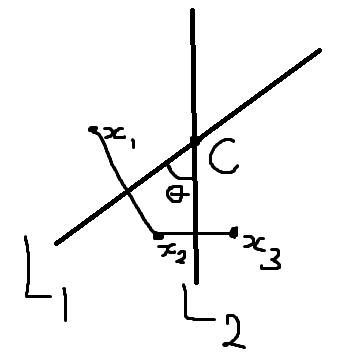
\includegraphics{Photos/Thingy.png}}\newline This drawing shows the process, the rotation is always clockwise. (Even if you start with $L_2$)
                \item Show that the composition of two reflections in parallel lines is a translation parallel to the lines and through twice the perpendicular distance between the lines.\myskip WLOG let $L_1$ and $L_2$ be horizontal lines going through the origin and $(0,d)$, respectively. Then any reflection in these lines will also be a horizontal line, thus it is parallel, and the point on the $y$-axis that it goes through is $(0,2d)$.
                \item Show that any isometry of $\R^2$ is a product of at most 3 reflections.\begin{proof}
                This is equivalent to saying any isometry can be generated by 3 non-colinear points. So, consider 3 arbitrary non-colinear points $A,B,C$, and an isometry between them, sending $A\mapsto A'$, $B\mapsto B'$, $C\mapsto C'$. Now, define $A$ to be the origin, and rotate about it until $AB$ is parallel to $A'B'$, if $AB$ is oriented incorrectly, use a reflection (or glide reflection) to line them up, finally, we use a translation to move $A$ onto $A'$.
                \end{proof}Again I'll use my trusty MS Paint to illustrate:\newline\scalebox{.5}{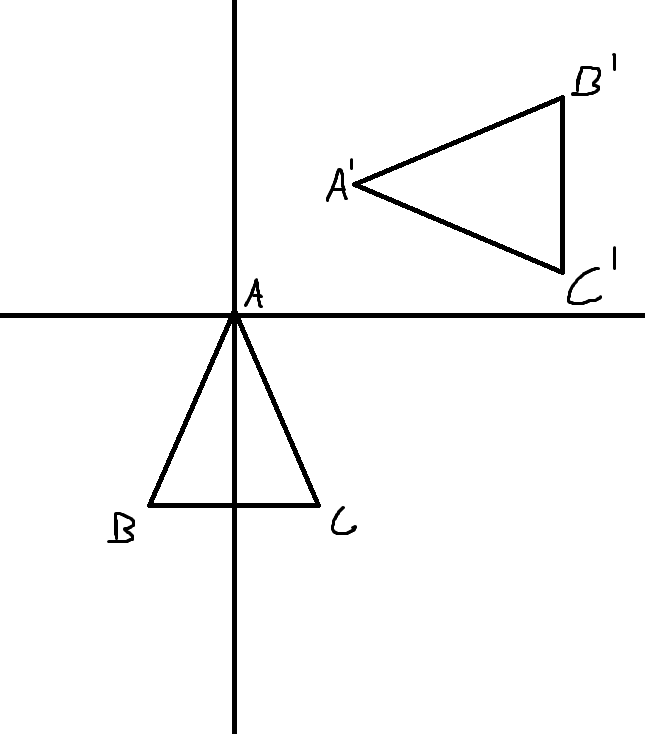
\includegraphics{Photos/Thing1.png}}\newline First step: rotate about $A$ until $AB$ is parallel to $A'B'$: \newline\scalebox{.5}{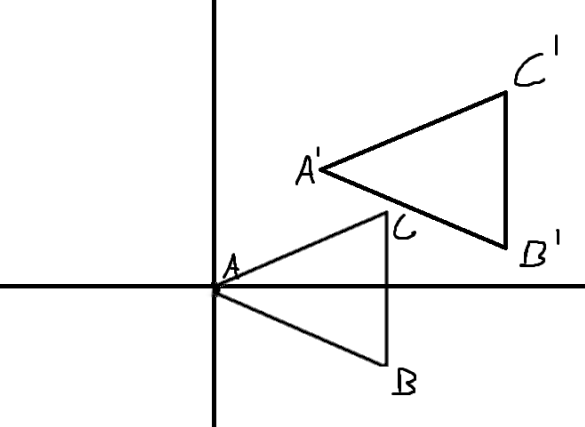
\includegraphics{Photos/Thing2.png}}\newline The final step is to translate $A$ onto $A'$, which will also align all the other points.\newline\scalebox{.5}{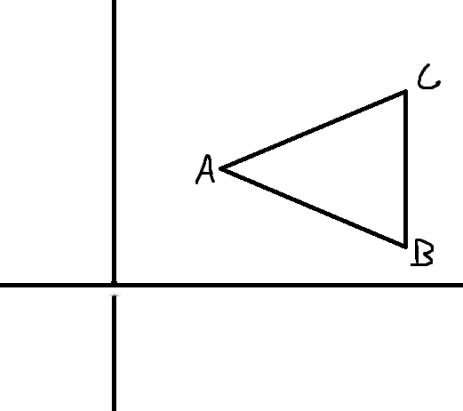
\includegraphics{Photos/Thing3.png}}
            \end{enumerate}
\end{document}